% generated by GAPDoc2LaTeX from XML source (Frank Luebeck)
\documentclass[a4paper,11pt]{report}
\usepackage{graphicx}
\usepackage{pgf}
\usepackage{tikz}
\usepgfmodule{plot}
\usepgflibrary{plothandlers}
\usetikzlibrary{shapes.geometric}
\usetikzlibrary{shadings}
\usepackage{a4wide}
\sloppy
\pagestyle{myheadings}
\usepackage{amssymb}
\usepackage[latin1]{inputenc}
\usepackage{makeidx}
\makeindex
\usepackage{color}
\definecolor{FireBrick}{rgb}{0.5812,0.0074,0.0083}
\definecolor{RoyalBlue}{rgb}{0.0236,0.0894,0.6179}
\definecolor{RoyalGreen}{rgb}{0.0236,0.6179,0.0894}
\definecolor{RoyalRed}{rgb}{0.6179,0.0236,0.0894}
\definecolor{LightBlue}{rgb}{0.8544,0.9511,1.0000}
\definecolor{Black}{rgb}{0.0,0.0,0.0}

\definecolor{linkColor}{rgb}{0.0,0.0,0.554}
\definecolor{citeColor}{rgb}{0.0,0.0,0.554}
\definecolor{fileColor}{rgb}{0.0,0.0,0.554}
\definecolor{urlColor}{rgb}{0.0,0.0,0.554}
\definecolor{promptColor}{rgb}{0.0,0.0,0.589}
\definecolor{brkpromptColor}{rgb}{0.589,0.0,0.0}
\definecolor{gapinputColor}{rgb}{0.589,0.0,0.0}
\definecolor{gapoutputColor}{rgb}{0.0,0.0,0.0}

%%  for a long time these were red and blue by default,
%%  now black, but keep variables to overwrite
\definecolor{FuncColor}{rgb}{0.0,0.0,0.0}
%% strange name because of pdflatex bug:
\definecolor{Chapter }{rgb}{0.0,0.0,0.0}
\definecolor{DarkOlive}{rgb}{0.1047,0.2412,0.0064}


\usepackage{fancyvrb}

\usepackage{mathptmx,helvet}
\usepackage[T1]{fontenc}
\usepackage{textcomp}


\usepackage[
            pdftex=true,
            bookmarks=true,        
            a4paper=true,
            pdftitle={Written with GAPDoc},
            pdfcreator={LaTeX with hyperref package / GAPDoc},
            colorlinks=true,
            backref=page,
            breaklinks=true,
            linkcolor=linkColor,
            citecolor=citeColor,
            filecolor=fileColor,
            urlcolor=urlColor,
            pdfpagemode={UseNone}, 
           ]{hyperref}

\newcommand{\maintitlesize}{\fontsize{50}{55}\selectfont}

% write page numbers to a .pnr log file for online help
\newwrite\pagenrlog
\immediate\openout\pagenrlog =\jobname.pnr
\immediate\write\pagenrlog{PAGENRS := [}
\newcommand{\logpage}[1]{\protect\write\pagenrlog{#1, \thepage,}}
%% were never documented, give conflicts with some additional packages

\newcommand{\GAP}{\textsf{GAP}}

%% nicer description environments, allows long labels
\usepackage{enumitem}
\setdescription{style=nextline}

%% depth of toc
\setcounter{tocdepth}{1}





%% command for ColorPrompt style examples
\newcommand{\gapprompt}[1]{\color{promptColor}{\bfseries #1}}
\newcommand{\gapbrkprompt}[1]{\color{brkpromptColor}{\bfseries #1}}
\newcommand{\gapinput}[1]{\color{gapinputColor}{#1}}


\begin{document}

\logpage{[ 0, 0, 0 ]}
\begin{titlepage}
\mbox{}\vfill

\begin{center}{\maintitlesize \textbf{\href{http://www.fc.up.pt/cmup/mdelgado/intpic} {IntPic}\mbox{}}}\\
\vfill

\hypersetup{pdftitle=\href{http://www.fc.up.pt/cmup/mdelgado/intpic} {IntPic}}
\markright{\scriptsize \mbox{}\hfill \href{http://www.fc.up.pt/cmup/mdelgado/intpic} {IntPic} \hfill\mbox{}}
{\Huge \textbf{A \textsf{GAP} package for drawing sets of integers\mbox{}}}\\
\vfill

{\Huge Version 0.1.0\mbox{}}\\[1cm]
{07 July 2013\mbox{}}\\[1cm]
\mbox{}\\[2cm]
{\Large \textbf{Manuel Delgado   \mbox{}}}\\
\hypersetup{pdfauthor=Manuel Delgado   }
\end{center}\vfill

\mbox{}\\
{\mbox{}\\
\small \noindent \textbf{Manuel Delgado   }  Email: \href{mailto://mdelgado@fc.up.pt} {\texttt{mdelgado@fc.up.pt}}\\
  Homepage: \href{http://cmup.fc.up.pt/cmup/mdelgado/} {\texttt{http://cmup.fc.up.pt/cmup/mdelgado/}}}\\
\end{titlepage}

\newpage\setcounter{page}{2}
{\small 
\section*{Copyright}
\logpage{[ 0, 0, 1 ]}
 \index{License} {\copyright} 2013 Manuel Delgado

 \noindent \href{http://www.fc.up.pt/cmup/mdelgado/intpic} {IntPic} package is free software; you can redistribute it and/or modify it under the
terms of the \href{http://www.fsf.org/licenses/gpl.html} {GNU General Public License} as published by the Free Software Foundation; either version 2 of the License,
or (at your option) any later version. For details, see the file 'GPL' in the
'etc' directory of the GAP distribution or see the FSF's own site. \mbox{}}\\[1cm]
{\small 
\section*{Acknowledgements}
\logpage{[ 0, 0, 3 ]}
 The author was partially funded by the European Regional Development Fund
through the program COMPETE and by the Portuguese Government through the FCT -
Funda{\c c}{\~a}o para a Ci{\^e}ncia e a Tecnologia under the project
PEst-C/MAT/UI0144/2011. 

 He benefited also of the sabbatical grant SFRH/BSAB/1156/2011. 

 Furthermore, I want to thank my colleagues of the Mathematics Department of
the Faculty of Sciences of the University of Porto for the opportunity of
taking a sabbatical year during the 2011/2012 school year. 

 For one reason or another that ranges from suggestions to encouragement, I
want express my gratitude to Pedro A. Garc{\a'\i}a S{\a'a}nchez, David Llena
and James Mitchell. \mbox{}}\\[1cm]
{\small 
\section*{Colophon}
\logpage{[ 0, 0, 2 ]}
 This manual describes the \textsf{GAP} package \href{http://www.fc.up.pt/cmup/mdelgado/intpic} {IntPic} version 0.1.0 for visualizing and creating publication quality pictures of
sets of integers. \mbox{}}\\[1cm]
\newpage

\def\contentsname{Contents\logpage{[ 0, 0, 4 ]}}

\tableofcontents
\newpage

  
\chapter{\textcolor{Chapter }{ The \textsf{IntPic} package }}\label{intro}
\logpage{[ 1, 0, 0 ]}
\hyperdef{L}{X82D13909840AC894}{}
{
   
\section{\textcolor{Chapter }{Overview and Introduction}}\logpage{[ 1, 1, 0 ]}
\hyperdef{L}{X87F9EA0A83C0DC65}{}
{
  The \href{http://www.fc.up.pt/cmup/mdelgado/intpic} {IntPic} package has as its main goal producing \texttt{Tikz} code for arrays of integers to be included in a {\LaTeX} file, which can then be processed. Some of the integers are emphasized, by
using different colors for the cells.  

 \href{http://www.fc.up.pt/cmup/mdelgado/intpic} {IntPic} grew up from my will to have a pictorial view of some sets of integers. I
wanted, in particular, get a pictorial view of the results produced by the \href{http://www.fc.up.pt/cmup/mdelgado/numericalsgps} {NumericalSgps} package \cite{DelgadoGarcia-SanchezMorais:numericalsgps}. Effort has then been made to serve a slightly more general purpose. For
instance, if the user wants to have a pictorial idea of how many primes there
are between 800 and 1000, or show it to his students and, perhaps, which among
these primes are twin primes, he will probably be happy by producing a picture
like the following 

  \begin{center}
\includegraphics[width=0.95\textwidth]{../images/primesandtwins} \end{center}   It has clearly too much information, given through the different colors. The
twin primes in the given range are in red-blue, while the remaining primes in
the same range are in red. 

 This package contains relatively few lines of code. The heavier part is the
documentation, where many examples are presented. 

 The design of this greatly benefits from my long experience on producing
visualization tools for \textsf{GAP} objects. The package \textsf{sgpviz} \cite{DelgadoMorais:sgpviz} is the visible part. More recently, I got involved in a more general project,
the \href{https://bitbucket.org/zen154115/viz} {Viz} package \cite{DelgadoEgri-NagyMitchellPfeiffer2012-Viz}. The experience gained there, especially through long and fruitful
discussions with J. Mitchell, influenced me a lot. This package will probably
be part of that more general project. For the moment it is independent, but
its use in conjunction with the \href{https://bitbucket.org/zen154115/viz} {Viz} package is recommended since in this case an immediate visualization is
provided. 

 The package produces \texttt{tikz} code that the user may then use at his wish. In particular, he can use it in
publications. But prior to obtaining results that lead to a publication, the
user may benefit of viewing thousands of images. There is a (almost platform
independent) function in \href{https://bitbucket.org/zen154115/viz} {Viz} that is intended to make this task easy. It benefits from the \textsf{GAP} stuff on creating a temporary directory where the computations occur. The
cleaning task is also left to \textsf{GAP}, which leaves the user free of the need of collecting the garbage. In order
to produce the drawings, {\LaTeX}, as well as some {\LaTeX} packages, in particular \texttt{tikz} and \texttt{pgf}, must be installed and working. I will assume that this is the case. All the
images in \cite{fengraoab} have been produced by using the \href{http://www.fc.up.pt/cmup/mdelgado/intpic} {IntPic} package. 

 This package consists basically of a function with many options associated.
The purpose of the manual is to illustrate the use of the options. Many
examples are presented. A file, named \texttt{examples.g} contains the \textsf{GAP} code, including the one to save the \texttt{tikz} code, to produce the examples in the manual. }

  
\section{\textcolor{Chapter }{ Installing \textsf{IntPic} }}\label{install}
\logpage{[ 1, 2, 0 ]}
\hyperdef{L}{X78F84769822AF0CB}{}
{
  In this section we give a brief description of how to start using \href{http://www.fc.up.pt/cmup/mdelgado/intpic} {IntPic}. If you have any problems getting \href{http://www.fc.up.pt/cmup/mdelgado/intpic} {IntPic} working, then you could try emailing me at \href{mailto://mdelgado@fc.up.pt} {\texttt{mdelgado@fc.up.pt}}. 

 It is assumed that you have a working copy of \textsf{GAP} with version number 4.5 or higher. The most up-to-date version of \textsf{GAP} and instructions on how to install it can be obtained from the main \textsf{GAP} web page \noindent\vspace{\baselineskip} \href{http://www.gap-system.org} {\texttt{http://www.gap-system.org}}. 

 \noindent If the \href{http://www.fc.up.pt/cmup/mdelgado/intpic} {IntPic} package was obtained as a part of the \textsf{GAP} distribution from the ``Download'' section of the \textsf{GAP} website, you may proceed to Section \ref{loading}. Alternatively, the \href{http://www.fc.up.pt/cmup/mdelgado/intpic} {IntPic} package may be installed using a separate archive, for example, for an update
or an installation in a non-default location (see  (\textbf{Reference: GAP Root Directories})). 

 Below we describe the installation procedure for the \texttt{.tar.gz} archive format, which can be obtained from \href{http://cmup.fc.up.pt/cmup/mdelgado/intpic/} {\texttt{http://cmup.fc.up.pt/cmup/mdelgado/intpic/}}. Installation using other archive formats or non UNIX-like systems is
performed in a similar way. 

 To install the \href{http://www.fc.up.pt/cmup/mdelgado/intpic} {IntPic} package, unpack the archive file, which should have a name of the form \texttt{ intpic-\mbox{\texttt{\mdseries\slshape XXX}}.tar.gz } for some version number \mbox{\texttt{\mdseries\slshape XXX}}, by typing 

 {\nobreakspace}{\nobreakspace} \texttt{ gzip -dc intpic-\mbox{\texttt{\mdseries\slshape XXX}}.tar.gz | tar xpv } 

 It may be unpacked in one of the following locations: 
\begin{itemize}
\item  in the \texttt{pkg} directory of your \textsf{GAP} installation; 
\item  or in a directory named \texttt{.gap/pkg} in your home directory (to be added to the \textsf{GAP} root directory unless \textsf{GAP} is started with \texttt{-r} option); 
\item  or in a directory named \texttt{pkg} in another directory of your choice (e.g.{\nobreakspace}in the directory \texttt{mygap} in your home directory). 
\end{itemize}
 In the latter case one must start \textsf{GAP} with the \texttt{-l} option, e.g.{\nobreakspace}if your private \texttt{pkg} directory is a subdirectory of \texttt{mygap} in your home directory you might type: 

 {\nobreakspace}{\nobreakspace} \texttt{ gap -l "\mbox{\texttt{\mdseries\slshape ;myhomedir}}/mygap" } 

 \noindent where \mbox{\texttt{\mdseries\slshape myhomedir}} is the path to your home directory, which may be replaced by a tilde (the
empty path before the semicolon is filled in by the default path of the \textsf{GAP} home directory). }

  
\section{\textcolor{Chapter }{ Loading \textsf{IntPic} }}\label{loading}
\logpage{[ 1, 3, 0 ]}
\hyperdef{L}{X7C04A5B97C484BB9}{}
{
  To use the \href{http://www.fc.up.pt/cmup/mdelgado/intpic} {IntPic} Package you have to request it explicitly. This is done by calling \texttt{LoadPackage} (\textbf{Reference: LoadPackage}): 

 
\begin{Verbatim}[commandchars=!@|,fontsize=\small,frame=single,label=Example]
  !gapprompt@gap>| !gapinput@LoadPackage("intpic");|
\end{Verbatim}
 

 The package banner, followed by \texttt{true}, will be shown, if the load has been successful. 

 If you want to load the \href{http://www.fc.up.pt/cmup/mdelgado/intpic} {IntPic} package by default, you can put the \texttt{LoadPackage} command into your \texttt{gaprc} file (see Section{\nobreakspace} (\textbf{Reference: The gap.ini and gaprc files})). }

 }

  
\chapter{\textcolor{Chapter }{ The \textsf{IntPic} package main function }}\label{functions}
\logpage{[ 2, 0, 0 ]}
\hyperdef{L}{X8769CA3686E2EDB7}{}
{
   This chapter consists of two sections, the first of which decribes the main
function of the package. The second one can be thought just as an example to
produce a table where the integers appear ordered in a non standard way. 
\section{\textcolor{Chapter }{The main function}}\logpage{[ 2, 1, 0 ]}
\hyperdef{L}{X80ABA2918548E108}{}
{
  The function \texttt{IP{\textunderscore}TikzArrayOfIntegers} (\ref{IPTikzArrayOfIntegers}) is the main function of the \href{http://www.fc.up.pt/cmup/mdelgado/intpic} {IntPic} package. It aims to produce \texttt{tikz} code for displaying arrays of integers. 
\subsection{\textcolor{Chapter }{Tikz code for arrays of integers}}\logpage{[ 2, 1, 1 ]}
\hyperdef{L}{X858D6CD18272C90F}{}
{
\noindent\textcolor{FuncColor}{$\triangleright$\ \ \texttt{IP{\textunderscore}TikzArrayOfIntegers({\mdseries\slshape arg})\index{IPTikzArrayOfIntegers@\texttt{IP{\textunderscore}}\-\texttt{Tikz}\-\texttt{Array}\-\texttt{Of}\-\texttt{Integers}}
\label{IPTikzArrayOfIntegers}
}\hfill{\scriptsize (function)}}\\


 The arguments (at most 3) are: 
\begin{enumerate}
\item (optional)
\begin{itemize}
\item  a table of integers. In this case, the length of the rows is the maximum of
the lengths of the sublists in the table, \emph{or} 
\item  a list of integers and, optionally, an integer which indicates the length of
the rows; when the length of the rows is not indicated, a compromise between
the width and the height is tried.
\end{itemize}

\item  a record of options. One of the fields of this record, named \texttt{highlights}, is an array whose entries are the numbers to be highlighted: one color per
sublist. See details and other options in Chapter{\nobreakspace}\ref{options}. 
\end{enumerate}
 When no list nor table is present, the smallest range containing all the
integers to be highlighted is taken. }

 
\begin{Verbatim}[commandchars=!@|,fontsize=\small,frame=single,label=Example]
  !gapprompt@gap>| !gapinput@rg := [81..89];;|
  !gapprompt@gap>| !gapinput@len := 10;;|
  !gapprompt@gap>| !gapinput@arr := [Filtered(rg,IsPrime),Filtered(rg,u->(u mod 2)=0),|
  !gapprompt@>| !gapinput@        Filtered(rg,u->(u mod 3)=0)];;|
  !gapprompt@gap>| !gapinput@tkz := IP_TikzArrayOfIntegers(rg,len,rec(highlights:=arr));;|
\end{Verbatim}
 The aspect of the string \mbox{\texttt{\mdseries\slshape tkz}} produced is not very appealing. We show it once, by asking it exlicitly in the
next example. In the forthcomming examples we keep using two semicolons to
avoid showing this kind of strings. 

 
\begin{Verbatim}[fontsize=\small,frame=single,label=The tkz string]
  gap> tkz;
  "%tikz\n\\begin{tikzpicture}[every node/.style={draw,scale=1pt,\nminimum width\
  =20pt,inner sep=3pt,\nline width=1pt,draw=black}]\n\\matrix[row sep=2pt,column\
   sep=2pt]\n{\\node[fill=-red]{86};&\n\\node[fill=green]{87};&\n\\node[fill=-re\
  d]{88};&\n\\node[fill=red]{89};\\\\\n\\node[fill=green]{81};&\n\\node[fill=-re\
  d]{82};&\n\\node[fill=red]{83};&\n\\node[left color=-red,right color=green]{84\
  };&\n\\node[]{85};\\\\\n};\n\\end{tikzpicture}\n"
\end{Verbatim}
 This string can be used at the users wish. In particular, it can be sent to
the standard output using the command \texttt{Print} (\textbf{Reference: Print}). 
\begin{Verbatim}[fontsize=\small,frame=single,label=The tikz code]
  gap> Print(tkz);
  %tikz
  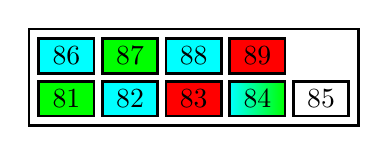
\begin{tikzpicture}[every node/.style={draw,scale=1pt,
  minimum width=20pt,inner sep=3pt,
  line width=1pt,draw=black}]
  \matrix[row sep=2pt,column sep=2pt]
  {\node[fill=-red]{86};&
  \node[fill=green]{87};&
  \node[fill=-red]{88};&
  \node[fill=red]{89};\\
  \node[fill=green]{81};&
  \node[fill=-red]{82};&
  \node[fill=red]{83};&
  \node[left color=-red,right color=green]{84};&
  \node[]{85};\\
  };
  \end{tikzpicture}
\end{Verbatim}
 It can now be copied and pasted in a {\LaTeX} document (having the appropriate packages in the preamble). See Chapter \ref{visualisation} for details and alternatives. 

  The next function uses the previous one, but is called with a simpler
argument. It will hopefully be useful for simple drawings. The length of each
row and the umber of columns varies. A compromise based on some experiments
has been established in order to obtain not too large nor too high images. 
\subsection{\textcolor{Chapter }{Tikz code for arrays, in a simplified way}}\logpage{[ 2, 1, 2 ]}
\hyperdef{L}{X7D3BCADE7903D62D}{}
{


 \noindent\textcolor{FuncColor}{$\triangleright$\ \ \texttt{IP{\textunderscore}SimpleTikzArrayOfIntegers({\mdseries\slshape arg})\index{IPSimpleTikzArrayOfIntegers@\texttt{IP{\textunderscore}}\-\texttt{Simple}\-\texttt{Tikz}\-\texttt{Array}\-\texttt{Of}\-\texttt{Integers}}
\label{IPSimpleTikzArrayOfIntegers}
}\hfill{\scriptsize (function)}}\\


 The argument is either a list of integers or a matrix of integers. The
integers involved are embeded in a range \mbox{\texttt{\mdseries\slshape rg}} of minimum length and highlighted by using the list of default colors. }

 
\begin{Verbatim}[commandchars=!@|,fontsize=\small,frame=single,label=Example]
  !gapprompt@gap>| !gapinput@d := DivisorsInt(30);|
  [ 1, 2, 3, 5, 6, 10, 15, 30 ]
  !gapprompt@gap>| !gapinput@IP_SimpleTizkArrayOfIntegers(d);;|
\end{Verbatim}
  \begin{center} \includegraphics[width=0.95\textwidth]{../images/divs30}
\end{center}   
\begin{Verbatim}[commandchars=!@|,fontsize=\small,frame=single,label=Example]
  !gapprompt@gap>| !gapinput@d30 := DivisorsInt(30);|
  [ 1, 2, 3, 5, 6, 10, 15, 30 ]
  !gapprompt@gap>| !gapinput@d40 := DivisorsInt(40);|
  [ 1, 2, 4, 5, 8, 10, 20, 40 ]
  !gapprompt@gap>| !gapinput@tkz := IP_SimpleTizkArrayOfIntegers([d30,d40]);;|
\end{Verbatim}
  \begin{center} \includegraphics[width=0.95\textwidth]{../images/divs3040}
\end{center}   

 }

  
\section{\textcolor{Chapter }{Producing tables}}\logpage{[ 2, 2, 0 ]}
\hyperdef{L}{X7EF12D7787D2A886}{}
{
  When the user is interested in tables of a certain kind, it may be a good idea
to write some code to produce these tables. The following function (whose code
is part of the file \emph{ip{\textunderscore}tables.gi} in the \emph{gap} folder of this package) is convenient to deal with numerical semigroups with
two generators and has been used to produce the images contained in \cite{fengraoab}. 

\subsection{\textcolor{Chapter }{IP{\textunderscore}TableWithModularOrder}}
\logpage{[ 2, 2, 1 ]}\nobreak
\hyperdef{L}{X816D055F845B0D71}{}
{\noindent\textcolor{FuncColor}{$\triangleright$\ \ \texttt{IP{\textunderscore}TableWithModularOrder({\mdseries\slshape o, a, b, depth, height, rep, pos})\index{IPTableWithModularOrder@\texttt{IP{\textunderscore}}\-\texttt{Table}\-\texttt{With}\-\texttt{Modular}\-\texttt{Order}}
\label{IPTableWithModularOrder}
}\hfill{\scriptsize (function)}}\\


 The arguments \mbox{\texttt{\mdseries\slshape rep}} and \mbox{\texttt{\mdseries\slshape pos}} are booleans (\texttt{true} or \texttt{false}). When \mbox{\texttt{\mdseries\slshape rep}} is \texttt{true} there is some repetition: the last column is equal to the first, but pushed
down some rows. When \mbox{\texttt{\mdseries\slshape pos}} is \texttt{true}, no rows below 0 are considered, (contradicting \mbox{\texttt{\mdseries\slshape depth}}, if needed). 

 The first five arguments arguments \mbox{\texttt{\mdseries\slshape o, a, b,depth}} and \mbox{\texttt{\mdseries\slshape height}} are integers. What they represent is described in what follows. There is
assigned some kind of a referential on the constructed table and the fist
argument, \mbox{\texttt{\mdseries\slshape o}}, stands for the origin. A table with \mbox{\texttt{\mdseries\slshape b}} columns ($\mbox{\texttt{\mdseries\slshape b}}+1$ columns when \mbox{\texttt{\mdseries\slshape rep}} is \texttt{true}) is constructed as follows. The row containing the origin is 
\begin{itemize}
\item $\mbox{\texttt{\mdseries\slshape o}}+ [0..\mbox{\texttt{\mdseries\slshape b}}-1]*\mbox{\texttt{\mdseries\slshape a}}$, if \mbox{\texttt{\mdseries\slshape rep}} is \texttt{false}, \emph{or}
\item $\mbox{\texttt{\mdseries\slshape o}}+ [0..\mbox{\texttt{\mdseries\slshape b}}]*\mbox{\texttt{\mdseries\slshape a}}$, if \mbox{\texttt{\mdseries\slshape rep}} is \texttt{true}
\end{itemize}
 

 The remaining rows are obtained by adding \mbox{\texttt{\mdseries\slshape b}} (the upper ones) or subtracting \mbox{\texttt{\mdseries\slshape b}} (the others) to these rows. 

 Note: when $\mbox{\texttt{\mdseries\slshape a}} < \mbox{\texttt{\mdseries\slshape b}}$ are co-prime, this construction provides a representation of the integers as
an array. 

 }

 
\begin{Verbatim}[commandchars=!@|,fontsize=\small,frame=single,label=Example]
  !gapprompt@gap>| !gapinput@a := 8;; b := 19;;  |
  !gapprompt@gap>| !gapinput@ns := NumericalSemigroup(a,b);;|
  !gapprompt@gap>| !gapinput@c := ConductorOfNumericalSemigroup(ns);;|
  !gapprompt@gap>| !gapinput@origin := 2*c-1;|
  251
  !gapprompt@gap>| !gapinput@ground := [origin..origin+b-1];;|
  !gapprompt@gap>| !gapinput@|
  !gapprompt@gap>| !gapinput@height:=2;;|
  !gapprompt@gap>| !gapinput@depth:=8;;|
  !gapprompt@gap>| !gapinput@  xaxis := [origin];;|
  !gapprompt@gap>| !gapinput@  for n in [1..b-1] do|
  !gapprompt@>| !gapinput@    Add(xaxis, origin+n*a);|
  !gapprompt@>| !gapinput@  od;|
  !gapprompt@gap>| !gapinput@  yaxis := [];;|
  !gapprompt@gap>| !gapinput@  for n in [-depth..height] do|
  !gapprompt@>| !gapinput@    Add(yaxis, origin+n*b);|
  !gapprompt@>| !gapinput@  od;|
  !gapprompt@gap>| !gapinput@|
  !gapprompt@gap>| !gapinput@table := TableWithModularOrder(origin,a,b,depth,height,false,false);;|
  !gapprompt@gap>| !gapinput@arr := [xaxis,yaxis,ground];|
  [ [ 251, 259, 267, 275, 283, 291, 299, 307, 315, 323, 331, 339, 347, 355, 
        363, 371, 379, 387, 395 ], 
    [ 99, 118, 137, 156, 175, 194, 213, 232, 251, 270, 289 ], [ 251 .. 269 ] ]
  !gapprompt@gap>| !gapinput@tkz:=IP_TikzArrayOfIntegers(table,rec(highlights:=arr));;|
\end{Verbatim}
  \begin{center}
\includegraphics[width=0.95\textwidth]{../images/table_axis_ground_8_19}
\end{center}   The next picture is obtained in the same way. The information that only the
shape has interest is given by including the option \texttt{shape{\textunderscore}only:=" "}. The variable \texttt{tkz} should be defined in a similar manner to the following one. 
\begin{Verbatim}[commandchars=@|B,fontsize=\small,frame=single,label=Example]
  @gapprompt|gap>B @gapinput|tkz:=IP_TikzArrayOfIntegers(table,rec(highlights:=arr,shape_only:=" ",B
  @gapprompt|>B @gapinput|             cell_width := "6",colsep:="1",rowsep:="1",inner_sep:="2",B
  @gapprompt|>B @gapinput|             line_color:="black!20"));;B
\end{Verbatim}
  \begin{center}
\includegraphics[width=0.80\textwidth]{../images/table_axis_ground_shape}
\end{center}   Next, a minimum of changes, just to illustrate the effect of \mbox{\texttt{\mdseries\slshape rep}} and \mbox{\texttt{\mdseries\slshape pos}}. 
\begin{Verbatim}[commandchars=!@|,fontsize=\small,frame=single,label=Example]
  !gapprompt@gap>| !gapinput@table := TableWithModularOrder(origin,a,b,depth,50,true,true);;|
  !gapprompt@gap>| !gapinput@tkz:=IP_TikzArrayOfIntegers(table,rec(highlights:=arr));;|
\end{Verbatim}
  \begin{center}
\includegraphics[width=0.80\textwidth]{../images/table_axis_ground_8_19_rep_pos}
\end{center}   }

 }

  
\chapter{\textcolor{Chapter }{ The colors in the \textsf{IntPic} package }}\label{colors}
\logpage{[ 3, 0, 0 ]}
\hyperdef{L}{X79D6BB838178DE6E}{}
{
   The idea in what concerns the colors is the following: the reader is free to
choose his colors (taking into account that the latex \textsf{xcolor} package is used), but we try to make users life reasonably easy. He is allowed
to choose tones. The default colors used by \href{http://www.fc.up.pt/cmup/mdelgado/intpic} {IntPic} are not many, although (from our experience) sufficient for most examples.  
\section{\textcolor{Chapter }{Colors by tones}}\logpage{[ 3, 1, 0 ]}
\hyperdef{L}{X85FF17E579A5481F}{}
{
  The colors are divided by tones.  
\begin{Verbatim}[fontsize=\small,frame=single,label=red]
  gap> IP_ColorsRedTones; #red
  [ "red", "red!50", "red!20", "red!80!green!50", "red!80!blue!60" ]
\end{Verbatim}
  \begin{center} \includegraphics[scale=1.2]{../images/red_tones.pdf}
\end{center}   
\begin{Verbatim}[fontsize=\small,frame=single,label=green]
  gap> IP_ColorsGreenTones; #green
  [ "green", "green!50", "green!20", "green!80!red!50", "green!80!blue!60" ]
\end{Verbatim}
  \begin{center} \includegraphics[scale=1.2]{../images/green_tones.pdf}
\end{center}   
\begin{Verbatim}[fontsize=\small,frame=single,label=blue]
  gap> IP_ColorsBlueTones; #blue
  [ "blue", "blue!50", "blue!20", "blue!80!red!50", "blue!80!green!60" ]
\end{Verbatim}
  \begin{center} \includegraphics[scale=1.2]{../images/blue_tones.pdf}
\end{center}   
\begin{Verbatim}[fontsize=\small,frame=single,label=cyan]
  gap> IP_ColorsCompRedTones; # cyan (complement of red)
  [ "-red", "-red!50", "-red!20", "-red!80!green!50", "-red!80!blue!60" ]
\end{Verbatim}
  \begin{center} \includegraphics[scale=1.2]{../images/comp_red_tones.pdf}
\end{center}   
\begin{Verbatim}[fontsize=\small,frame=single,label=magenta]
  gap> IP_ColorsCompGreenTones; # magenta (complement of green)
  [ "-green", "-green!50", "-green!20", "-green!80!red!50", "-green!80!blue!60" 
   ]
\end{Verbatim}
  \begin{center} \includegraphics[scale=1.2]{../images/comp_green_tones.pdf}
\end{center}   
\begin{Verbatim}[fontsize=\small,frame=single,label=yellow]
  gap> IP_ColorsCompBlueTones; # yellow (complement of blue)
  [ "-blue", "-blue!50", "-blue!20", "-blue!80!red!50", "-blue!80!green!60" ]
\end{Verbatim}
  \begin{center} \includegraphics[scale=1.2]{../images/comp_blue_tones.pdf}
\end{center}   
\begin{Verbatim}[fontsize=\small,frame=single,label=dark gray]
  gap> IP_ColorsDGrayTones; # dark gray
  [ "black!80", "black!70", "black!60", "black!50", "black!40" ]
\end{Verbatim}
  \begin{center} \includegraphics[scale=1.2]{../images/dark_gray_tones.pdf}
\end{center}   
\begin{Verbatim}[fontsize=\small,frame=single,label=light gray]
  gap> IP_ColorsLGrayTones; # light gray
  [ "black!30", "black!25", "black!20", "black!15", "black!10" ]
\end{Verbatim}
  \begin{center} \includegraphics[scale=1.2]{../images/light_gray_tones.pdf}
\end{center}   }

 
\section{\textcolor{Chapter }{Lists of colors}}\logpage{[ 3, 2, 0 ]}
\hyperdef{L}{X835CFDFB7C27CC26}{}
{
  
\begin{Verbatim}[fontsize=\small,frame=single,label=array of colors by tones]
  gap> ListsOfIP_Colors;
  [ [ "red", "red!50", "red!20", "red!80!green!50", "red!80!blue!60" ], 
    [ "green", "green!50", "green!20", "green!80!red!50", "green!80!blue!60" ], 
    [ "blue", "blue!50", "blue!20", "blue!80!red!50", "blue!80!green!60" ], 
    [ "-red", "-red!50", "-red!20", "-red!80!green!50", "-red!80!blue!60" ], 
    [ "-green", "-green!50", "-green!20", "-green!80!red!50", 
        "-green!80!blue!60" ], 
    [ "-blue", "-blue!50", "-blue!20", "-blue!80!red!50", "-blue!80!green!60" ],
    [ "black!80", "black!70", "black!60", "black!50", "black!40" ], 
    [ "black!30", "black!25", "black!20", "black!15", "black!10" ] ]
\end{Verbatim}
 
\begin{Verbatim}[fontsize=\small,frame=single,label=list of colors by tones]
  gap> IP_Colors;
  [ "red", "red!50", "red!20", "red!80!green!50", "red!80!blue!60", "green", 
    "green!50", "green!20", "green!80!red!50", "green!80!blue!60", "blue", 
    "blue!50", "blue!20", "blue!80!red!50", "blue!80!green!60", "-red", 
    "-red!50", "-red!20", "-red!80!green!50", "-red!80!blue!60", "-green", 
    "-green!50", "-green!20", "-green!80!red!50", "-green!80!blue!60", "-blue", 
    "-blue!50", "-blue!20", "-blue!80!red!50", "-blue!80!green!60", "black!80", 
    "black!70", "black!60", "black!50", "black!40", "black!30", "black!25", 
    "black!20", "black!15", "black!10" ]
\end{Verbatim}
 }

 
\section{\textcolor{Chapter }{The \textsf{IntPic} default list of colors}}\logpage{[ 3, 3, 0 ]}
\hyperdef{L}{X80B1B11779AA0CB6}{}
{
  The colors are shuffled by concatenating the transposed of the matrix \texttt{ListsOfIP{\textunderscore}Colors}. The list obtained is taken as the default list of colors. 
\begin{Verbatim}[fontsize=\small,frame=single,label=default list of colors]
  gap> ShuffledIP_colors;
  [ "red", "green", "blue", "-red", "-green", "-blue", "black!80", "black!30", 
    "red!50", "green!50", "blue!50", "-red!50", "-green!50", "-blue!50", 
    "black!70", "black!25", "red!20", "green!20", "blue!20", "-red!20", 
    "-green!20", "-blue!20", "black!60", "black!20", "red!80!green!50", 
    "green!80!red!50", "blue!80!red!50", "-red!80!green!50", "-green!80!red!50",
    "-blue!80!red!50", "black!50", "black!15", "red!80!blue!60", 
    "green!80!blue!60", "blue!80!green!60", "-red!80!blue!60", 
    "-green!80!blue!60", "-blue!80!green!60", "black!40", "black!10" ]
\end{Verbatim}
  \begin{center}
\includegraphics[width=0.8\textwidth]{../images/intpic_default_colors.pdf}
\end{center}   These are the \href{http://www.fc.up.pt/cmup/mdelgado/intpic} {IntPic} default colors. Although the user is free to use other colors, we warn that
there is a need of compatibility with the colors used in other packages (the {\LaTeX} \textsf{xcolor}, for instance). To emphasize the integers of some sets by using some of the
colors in some list of colors (for instance the default colors) one may use
empty lists to force the non usage of the colors whose order in the list of
colors is the order of these empty lists in the array of integers to be
emphasized. 
\begin{Verbatim}[commandchars=!@|,fontsize=\small,frame=single,label=Example]
  !gapprompt@gap>| !gapinput@m3 := Filtered([1..40],i->i mod 3=0);|
  [ 3, 6, 9, 12, 15, 18, 21, 24, 27, 30, 33, 36, 39 ]
  !gapprompt@gap>| !gapinput@m5 := Filtered([1..40],i->i mod 5=0);|
  [ 5, 10, 15, 20, 25, 30, 35, 40 ]
  !gapprompt@gap>| !gapinput@m7 := Filtered([1..40],i->i mod 7=0);|
  [ 7, 14, 21, 28, 35 ]
  !gapprompt@gap>| !gapinput@|
  !gapprompt@gap>| !gapinput@arr := [[],[],m3,[],m5,[],m7];;|
  !gapprompt@gap>| !gapinput@tkz:=IP_TikzArrayOfIntegers([1..40],10,rec(highlights:=arr));;|
\end{Verbatim}
  \begin{center} \includegraphics[width=0.8\textwidth]{../images/mults_3_5_7}
\end{center}   }

 
\section{\textcolor{Chapter }{Functions to deal with colors}}\logpage{[ 3, 4, 0 ]}
\hyperdef{L}{X7BD48BC279D8FDF4}{}
{
   For the moment we only provide one function, which shuffles colors from lists
of colors. 
\subsection{\textcolor{Chapter }{Shuffle colors from lists of colors}}\logpage{[ 3, 4, 1 ]}
\hyperdef{L}{X795C4D9A7B1A2600}{}
{
\noindent\textcolor{FuncColor}{$\triangleright$\ \ \texttt{ShuffleIP{\textunderscore}Colors({\mdseries\slshape mat})\index{ShuffleIPColors@\texttt{ShuffleIP{\textunderscore}Colors}}
\label{ShuffleIPColors}
}\hfill{\scriptsize (function)}}\\


 The argument \mbox{\texttt{\mdseries\slshape mat}} is a list of lists of colors of the same length. The output is obtained by
concatenating the transposed of \mbox{\texttt{\mdseries\slshape mat}}. 
\begin{Verbatim}[commandchars=@|A,fontsize=\small,frame=single,label=Example]
  @gapprompt|gap>A @gapinput|ShuffleIP_Colors([IP_ColorsRedTones,IP_ColorsCompBlueTones]);A
  [ "red", "-blue", "red!50", "-blue!50", "red!20", "-blue!20", 
    "red!80!green!50", "-blue!80!red!50", "red!80!blue!60", "-blue!80!green!60" 
   ]
\end{Verbatim}
  \begin{center}
\includegraphics[scale=1.2]{../images/shuffle_red_comp_blue.pdf} \end{center}   }

 }

 }

  
\chapter{\textcolor{Chapter }{Visualization of the pictures created}}\label{visualisation}
\logpage{[ 4, 0, 0 ]}
\hyperdef{L}{X79BE6CBC7AA29804}{}
{
  This chapter describes two easy ways to visualize the images created by using
the \href{http://www.fc.up.pt/cmup/mdelgado/intpic} {IntPic} package. Both require {\LaTeX} and some {\LaTeX} packages, such as \textsf{Tikz} and \textsf{pgf}, to be installed and working. One of the ways we will describe is almost
completely automatic, but requires the \href{https://bitbucket.org/zen154115/viz} {Viz} package. The other is not so automatic but has the advantage of not requiring
other packages, besides the {\LaTeX} ones. 

  
\section{\textcolor{Chapter }{Viewing using \textsf{Viz}}}\logpage{[ 4, 1, 0 ]}
\hyperdef{L}{X78668CD6797F734B}{}
{
  If you have a working copy of the \href{https://bitbucket.org/zen154115/viz} {Viz} package, you may produce and display a picture from a \texttt{tikz} string \mbox{\texttt{\mdseries\slshape tkz}} just by typing the following: 

 

 
\begin{Verbatim}[fontsize=\small,frame=single,label=Splash]
  Splash(tkz);
\end{Verbatim}
 A picture is popped up after this use of the function \texttt{Splash} (\textbf{Viz: Splash}). To see the name of the temporary directory created to perform the
computations, and thus being able to copy the files involved to any other
place, one should set the info level \texttt{InfoViz} to $1$ or more. The following example illustrates this and the use of some options of
the \texttt{Splash} (\textbf{Viz: Splash}) function of the \href{https://bitbucket.org/zen154115/viz} {Viz} package. Setting the option \texttt{papersize} to "a0paper" may be convenient for the visualization of large images. The \texttt{pdf} viewer can also be changed. 
\begin{Verbatim}[fontsize=\small,frame=single,label=infoviz: temporary directory]
  gap> SetInfoLevel(InfoViz,1);
  gap> Splash(tkz,rec(latexpoints:="10pt",papersize:="a0paper",viewer:="okular")); 
  #I  The temporary directory used is: /tmp/tmJcpphI/
\end{Verbatim}
 The temporary directory /tmp/tmJcpphI/ contains the files vizpicture1.tex and
vizpicture.tex. The file vizpicture1.tex contains the tikz code and the file
vizpicture.tex is the {\LaTeX} document to be processed. Other files, namely the \texttt{vizpicture.pdf} are created by the \texttt{pdflatex} command that is called by the \texttt{Splash} (\textbf{Viz: Splash}) function. }

 
\section{\textcolor{Chapter }{Viewing without using \textsf{Viz}}}\logpage{[ 4, 2, 0 ]}
\hyperdef{L}{X7CED7CEA804873E1}{}
{
  This section describes a way to visualize images without sing \href{https://bitbucket.org/zen154115/viz} {Viz}. Besides being useful in the case of not having a working copy of \href{https://bitbucket.org/zen154115/viz} {Viz}, it is rather convenient when the decision of where to save the pictures is
made. In this case, you may start your gap session in the desired place, the
working directory. Furthermore, if your intention is, for instance, to include
the images in a document, you may just decide the name for the file containing
the \texttt{tikz} code and let your document input it. The glogal variables \texttt{IP{\textunderscore}Preamble} and \texttt{Closing} can be used to pruduce a complete {\LaTeX} document rather than only the \texttt{tizk} code for the picture. The document may then be processed by using \texttt{pdflatex} and the picture viewed by using some \texttt{pdf} viewer. The \texttt{pdf} produced can be included in a {\LaTeX} document instead of the \texttt{tizk} code. In the later case, the code is processed each time the document is
processed, which should perhaps be avoided in the case of large images. 

 Note the use of the \texttt{preview} package, which is used to produce the complete picture without having to pay
attention to the paper size nor to crop the image. It is useful for viewing
purposes and also to include the \texttt{pdf} file produced in a {\LaTeX} document to be processed with \texttt{pdflatex}. 
\begin{Verbatim}[fontsize=\small,frame=single,label=Preamble]
  gap> Print(IP_Preamble);
  \documentclass{minimal}
  \usepackage{amsmath}
  \usepackage[active,tightpage]{preview}
  \setlength\PreviewBorder{1pt}
  \usepackage{pgf}
  \usepackage{tikz}
  \usepgfmodule{plot}
  \usepgflibrary{plothandlers}
  \usetikzlibrary{shapes.geometric}
  \usetikzlibrary{shadings}
  \begin{document}
  \begin{preview}
\end{Verbatim}
 
\begin{Verbatim}[fontsize=\small,frame=single,label=Closing]
  gap> Print(IP_Closing);
  \end{preview}
  \end{document}
\end{Verbatim}
 
\subsection{\textcolor{Chapter }{A complete example}}\logpage{[ 4, 2, 1 ]}
\hyperdef{L}{X7B47AFA881BFC9DC}{}
{
  Admit you want to produce a document which contains the picture corresponding
to the \texttt{tikz} code obtained through the instructions 
\begin{Verbatim}[fontsize=\small,frame=single,label=instructions to obtain some tikz code]
  arr := [[1,2,3,4,5,6],[1,2,3,4,5],[1,2,3,4],[1,2,3],[1,2],[1]];;
  tkz := IP_TikzArrayOfIntegers([1..10],5,rec(highlights:=arr));;
\end{Verbatim}
 The picture is:  \begin{center}
\includegraphics[width=0.95\textwidth]{../images/pic_for_complete_document.pdf}
\end{center}   The elements of the set $[1,2,3,4,5,6]$ are highlighted using the first color (red); those of the set $[1,2,3,4,5]$ are highlighted using the second color (green); those of the set $[1,2,3,4]$ are highlighted using the third color (blue); those of the set $[1,2,3]$ are highlighted using the fourth color (cyan); those of the set $[1,2]$ are highlighted using the fifth color (magenta); those of the set $[1]$ is highlighted using the sixth color (yellow). 

 Let us explain how the six colors used for the cell containing $1$ are distributed: upper left corner -- red; upper right corner -- green; lower
left corner -- blue; lower right corner -- cyan; the number -- magenta; the
border -- yellow. 

 The colors of the cell containing $2$ and $3$ are distributed in a similar way. 

 The colors of the cell containing $4$: left -- red; middle -- blue; right -- green. 

 After the session listed below, the files \texttt{tikz{\textunderscore}pic{\textunderscore}for{\textunderscore}complete{\textunderscore}document.tex} and \texttt{pic{\textunderscore}for{\textunderscore}complete{\textunderscore}document.tex} have been created in the current directory (that is, the one where the \textsf{GAP} session has started). For other directories, complete paths may have to be
given. 
\begin{Verbatim}[fontsize=\small,frame=single,label=the GAP session]
  gap> tikzfile := "tikz_pic_for_complete_document.tex";;
  gap> file := "pic_for_complete_document.tex";;
  gap> 
  gap> arr := [[1,2,3,4,5,6],[1,2,3,4,5],[1,2,3,4],[1,2,3],[1,2],[1]];;
  gap> tkz := IP_TikzArrayOfIntegers([1..10],5,rec(highlights:=arr));;
  gap> 
  gap> FileString(tikzfile,tkz);
  642
  gap> FileString(file,Concatenation(IP_Preamble,tkz,IP_Closing));
  961
\end{Verbatim}
 Executing something like 
\begin{Verbatim}[fontsize=\small,frame=single,label=the pdf and the jpg of the picture]
  pdflatex pic_for_complete_document.tex
  convert pic_for_complete_document.pdf pic_for_complete_document.jpg
\end{Verbatim}
 the \texttt{pdf} and the \texttt{jpg} formats of the image have been created. The \texttt{jpg} format is usefull to be included into an html document, for instance. 

 Note that the tikz code has been saved into the file \texttt{tikz{\textunderscore}pic{\textunderscore}for{\textunderscore}complete{\textunderscore}document.tex}. A complete example of a {\LaTeX} document follows. 
\begin{Verbatim}[fontsize=\small,frame=single,label=a LaTeX document]
  \documentclass{article}
  \usepackage{amsmath}
  %\usepackage[active,tightpage]{preview}
  %\setlength\PreviewBorder{1pt}
  \usepackage{pgf}
  \usepackage{tikz}
  \usepgfmodule{plot}
  \usepgflibrary{plothandlers}
  \usetikzlibrary{shapes.geometric}
  \usetikzlibrary{shadings}
  \usepackage{graphicx}
  \author{Author}
  \title{How to include images in a \LaTeX\ document}
  \date{June, 2013}
  \begin{document}
  %\begin{preview}
  \maketitle
  Using the pdf file:
  
  \begin{center}
    \includegraphics[width=0.80\textwidth]{../images/pic_for_complete_document.pdf}
  \end{center}
  
  Using the PGF/TikZ code:
  
  \begin{center}
  %tikz
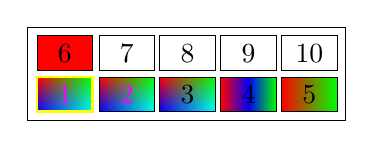
\begin{tikzpicture}[every node/.style={draw,scale=1pt,
minimum width=20pt,inner sep=3pt,
line width=0pt,draw=black}]
\matrix[row sep=2pt,column sep=2pt]
{\node[fill=red]{6};&
\node[]{7};&
\node[]{8};&
\node[]{9};&
\node[]{10};\\
\node[upper left=red,upper right=green,lower left=blue,lower right=-red,text=-green,thick,draw=-blue]{1};&
\node[,upper left=red,upper right=green,lower left=blue,lower right=-red,text=-green]{2};&
\node[,upper left=red,upper right=green,lower left=blue,lower right=-red]{3};&
\node[left color=red,right color=green,middle color=blue]{4};&
\node[left color=red,right color=green]{5};\\
};
\end{tikzpicture}

  \end{center}
  If you want to scale this immage, please chang the ``scale'' in the file
  \textt{tikz_pic_for_complete_document.tex} 
  %\end{preview}
  \end{document}
\end{Verbatim}
 The output, after processing with \texttt{pdflatex} is as follows:  \begin{center}
\includegraphics[width=0.95\textwidth]{../images/complete_latex_document.pdf}
\end{center}   }

 }

 
\section{\textcolor{Chapter }{Other examples of use of the \textsf{IntPic} package}}\logpage{[ 4, 3, 0 ]}
\hyperdef{L}{X831140698300DBD0}{}
{
  
\subsection{\textcolor{Chapter }{Varia}}\logpage{[ 4, 3, 1 ]}
\hyperdef{L}{X850A57EF80CDB124}{}
{
  The following example shows how to produce \texttt{tikz} code for a picture containing the odd integers from $801$ to $999$. Each line (except the highest) contains $15$ cells. 
\begin{Verbatim}[commandchars=!@|,fontsize=\small,frame=single,label=Example]
  !gapprompt@gap>| !gapinput@rg := Filtered([801..889],u->(u mod 2)<>0);;|
  !gapprompt@gap>| !gapinput@flen := 15;;|
  !gapprompt@gap>| !gapinput@twins := Filtered(Primes, p -> p + 2 in Primes);;|
  !gapprompt@gap>| !gapinput@arr := [Primes,Union(twins,twins+2),Filtered(rg,u->(u mod 3)=0)];;|
  !gapprompt@gap>| !gapinput@tkz := IP_TikzArrayOfIntegers(rg,flen,rec(highlights:=arr));;|
\end{Verbatim}
 The picture obtained highlights the primes, the twin primes and the multiples
of $3$. As the twins are also primes, a gradient is used to highlight them. In this
example the default list of colors is used.  \begin{center}
\includegraphics[width=0.95\textwidth]{../images/primesandtwinsamongodd}
\end{center}   The same computations, but defining other color lists. 
\begin{Verbatim}[commandchars=!@|,fontsize=\small,frame=single,label=Example]
  !gapprompt@gap>| !gapinput@cls := IP_ColorsCompRedTones;;|
  !gapprompt@gap>| !gapinput@rg := Filtered([801..889],u->(u mod 2)<>0);;|
  !gapprompt@gap>| !gapinput@flen := 15;;|
  !gapprompt@gap>| !gapinput@twins := Filtered(Primes, p -> p + 2 in Primes);;|
  !gapprompt@gap>| !gapinput@arr := [Primes,Union(twins,twins+2),Filtered(rg,u->(u mod 3)=0)];;|
  !gapprompt@gap>| !gapinput@tkz := IP_TikzArrayOfIntegers(rg,flen,rec(colors := cls,highlights:=arr));;|
\end{Verbatim}
  \begin{center}
\includegraphics[width=0.95\textwidth]{../images/primesandtwinsamongodd_comp_red}
\end{center}   
\begin{Verbatim}[commandchars=!@|,fontsize=\small,frame=single,label=Example]
  !gapprompt@gap>| !gapinput@cls := IP_ColorsDGrayTones;;|
  !gapprompt@gap>| !gapinput@rg := Filtered([801..889],u->(u mod 2)<>0);;|
  !gapprompt@gap>| !gapinput@flen := 15;;|
  !gapprompt@gap>| !gapinput@twins := Filtered(Primes, p -> p + 2 in Primes);;|
  !gapprompt@gap>| !gapinput@arr := [Primes,Union(twins,twins+2),Filtered(rg,u->(u mod 3)=0)];;|
  !gapprompt@gap>| !gapinput@tkz := IP_TikzArrayOfIntegers(rg,flen,rec(colors := cls,highlights:=arr));;|
\end{Verbatim}
  \begin{center}
\includegraphics[width=0.95\textwidth]{../images/primesandtwinsamongodd_dark_gray}
\end{center}   
\begin{Verbatim}[commandchars=!@|,fontsize=\small,frame=single,label=Example]
  !gapprompt@gap>| !gapinput@cls := ["blue","-blue","black"];;|
  !gapprompt@gap>| !gapinput@rg := Filtered([801..889],u->(u mod 2)<>0);;|
  !gapprompt@gap>| !gapinput@flen := 15;;|
  !gapprompt@gap>| !gapinput@twins := Filtered(Primes, p -> p + 2 in Primes);;|
  !gapprompt@gap>| !gapinput@arr := [Primes,Union(twins,twins+2),Filtered(rg,u->(u mod 3)=0)];;|
  !gapprompt@gap>| !gapinput@tkz := IP_TikzArrayOfIntegers(rg,flen,rec( colors := cls,highlights:=arr));;|
\end{Verbatim}
  \begin{center}
\includegraphics[width=0.95\textwidth]{../images/primesandtwinsamongodd_other}
\end{center}   The following example uses the  \href{http://www.fc.up.pt/cmup/mdelgado/numericalsgps} {NumericalSgps}   package. 
\begin{Verbatim}[commandchars=!@|,fontsize=\small,frame=single,label=Example]
  
  !gapprompt@gap>| !gapinput@#LoadPackage("numericalsgps");|
  !gapprompt@gap>| !gapinput@|
  !gapprompt@gap>| !gapinput@ns := NumericalSemigroup(11,19,30,42,59);;|
  !gapprompt@gap>| !gapinput@cls := ShuffleIP_Colors([IP_ColorsGreenTones,IP_ColorsCompBlueTones]);;|
  !gapprompt@gap>| !gapinput@flen := 20;;|
  !gapprompt@gap>| !gapinput@#some notable elements|
  !gapprompt@gap>| !gapinput@arr := [SmallElementsOfNumericalSemigroup(ns),|
  !gapprompt@>| !gapinput@        GapsOfNumericalSemigroup(ns),|
  !gapprompt@>| !gapinput@        MinimalGeneratingSystemOfNumericalSemigroup(ns),|
  !gapprompt@>| !gapinput@        FundamentalGapsOfNumericalSemigroup(ns),|
  !gapprompt@>| !gapinput@        [ConductorOfNumericalSemigroup(ns)],|
  !gapprompt@>| !gapinput@        PseudoFrobeniusOfNumericalSemigroup(ns)];;|
  !gapprompt@gap>| !gapinput@|
  !gapprompt@gap>| !gapinput@tkz := IP_TikzArrayOfIntegers(flen,rec(colors := cls,highlights:=arr));;|
\end{Verbatim}
  \begin{center}
\includegraphics[width=0.95\textwidth]{../images/numericalsgp_notable}
\end{center}   Using the default colors  \begin{center}
\includegraphics[width=0.95\textwidth]{../images/numericalsgp_notable_df_colors}
\end{center}   }

 
\subsection{\textcolor{Chapter }{The banner}}\logpage{[ 4, 3, 2 ]}
\hyperdef{L}{X784E0A5A7DB88332}{}
{
  The code in the following example has been used to produce one possible banner
for the homepage of the \href{http://www.fc.up.pt/cmup/mdelgado/intpic} {IntPic} package. It is a nice picture that gives an idea about the primes less than $10000$. Of course, other ranges could have been chosen. I warn the user that
pictures involving a large amount of data may face the problem of exceeding {\TeX} capacity... 
\begin{Verbatim}[commandchars=@|B,fontsize=\small,frame=single,label=Example]
  @gapprompt|gap>B @gapinput|row_length := 200;; # the legth of each rowB
  @gapprompt|gap>B @gapinput|columns := 50;; # the number of columsB
  @gapprompt|gap>B @gapinput|n := row_length*columns;B
  10000
  @gapprompt|gap>B @gapinput|B
  @gapprompt|gap>B @gapinput|##compute the primes less than nB
  @gapprompt|gap>B @gapinput|# Primes is a GAP variable representing the list of primes less than 1000B
  @gapprompt|gap>B @gapinput|mp := Maximum(Primes);B
  997
  @gapprompt|gap>B @gapinput|newprimes := [];;B
  @gapprompt|gap>B @gapinput|while mp < n doB
  @gapprompt|>B @gapinput|  mp := NextPrimeInt(mp);B
  @gapprompt|>B @gapinput|  Add(newprimes, mp);B
  @gapprompt|>B @gapinput|od;B
  @gapprompt|gap>B @gapinput|small_primes := Union(Primes, newprimes);;B
  @gapprompt|gap>B @gapinput|##compute the first element of each pair of twin primes less than nB
  @gapprompt|gap>B @gapinput|twins := Filtered(small_primes, p -> IsPrime(p+2));;B
  @gapprompt|gap>B @gapinput|B
  @gapprompt|gap>B @gapinput|rg := [1..n];;B
  @gapprompt|gap>B @gapinput|B
  @gapprompt|gap>B @gapinput|arr := [Intersection(small_primes,rg),[],[], B
  @gapprompt|>B @gapinput|        Intersection(Union(twins,twins+2),rg),[],[],[],[],[],[],[],B
  @gapprompt|>B @gapinput|        [],[],[],[],[],[],Difference(rg,small_primes)];;B
  @gapprompt|gap>B @gapinput|B
  @gapprompt|gap>B @gapinput|tkz:=IP_TikzArrayOfIntegers([1..n],row_length,rec(highlights:=arr,B
  @gapprompt|>B @gapinput|             cell_width := "6",colsep:="0",rowsep:="0",inner_sep:="2",B
  @gapprompt|>B @gapinput|             shape_only:=" ",line_width:="0",line_color:="black!20" ));;B
\end{Verbatim}
  \begin{center}
\includegraphics[width=0.99\textwidth]{../images/intpic_banner.pdf}
\end{center}   }

 }

 }

  
\chapter{\textcolor{Chapter }{ The \textsf{IntPic} package options. }}\label{options}
\logpage{[ 5, 0, 0 ]}
\hyperdef{L}{X8104F6457E34C76F}{}
{
  
\section{\textcolor{Chapter }{Available options}}\logpage{[ 5, 1, 0 ]}
\hyperdef{L}{X83F97BF484ED50E5}{}
{
  The list of allowed options, some of which already familiar from the examples,
can be obtained as follows: 
\begin{Verbatim}[commandchars=!@|,fontsize=\small,frame=single,label=Example]
  !gapprompt@gap>| !gapinput@RecNames(IP_TikzDefaultOptionsForArraysOfIntegers);|
  [ "other", "colors", "highlights", "shape_only", "colsep", "rowsep", 
    "cell_width", "allow_adjust_cell_width", "scale", "inner_sep", 
    "line_width", "line_color" ]
\end{Verbatim}
 Its meaning is as follows: 
\begin{itemize}
\item  \mbox{\texttt{\mdseries\slshape colors}}: any list of colors (to be used with the {\LaTeX} package \textsf{xcolor}) 
\item  \mbox{\texttt{\mdseries\slshape highlights}}: a list of lists of integers -- the elements of the first are colored by
using the first color, etc. In cases of elements that appear in more than one
list a kind of gradient (made with 4 colors at most) is used to fill the cell;
the number may be printed with a fifth color and a sixt color may be used for
the border. 
\item  \mbox{\texttt{\mdseries\slshape shape{\textunderscore}only}}: an option to be used when only the shape is important. When \mbox{\texttt{\mdseries\slshape true}} or " " is used, all the nodes are empty; using a symbol, for instance a $*$, this symbol is printed in all the nodes. 
\item  \mbox{\texttt{\mdseries\slshape colsep}}: the \textsf{tikz} matrix option \mbox{\texttt{\mdseries\slshape column sep}} 
\item  \mbox{\texttt{\mdseries\slshape rowsep}}: the \textsf{tikz} matrix option \mbox{\texttt{\mdseries\slshape row sep}} 
\item  \mbox{\texttt{\mdseries\slshape cell{\textunderscore}width}}: the \textsf{tikz} matrix option \mbox{\texttt{\mdseries\slshape minimum width}} 
\item  \mbox{\texttt{\mdseries\slshape scale}}: the \textsf{tikz} matrix option \mbox{\texttt{\mdseries\slshape scale}} 
\item  \mbox{\texttt{\mdseries\slshape inner{\textunderscore}sep}}: the \textsf{tikz} matrix option \mbox{\texttt{\mdseries\slshape inner sep}} 
\item  \mbox{\texttt{\mdseries\slshape line{\textunderscore}width}}: the \textsf{tikz} matrix option \mbox{\texttt{\mdseries\slshape line width}} 
\item  \mbox{\texttt{\mdseries\slshape line{\textunderscore}color}}: the \textsf{tikz} matrix option \mbox{\texttt{\mdseries\slshape line color}}: the color of the cell borders 
\item  \mbox{\texttt{\mdseries\slshape allow{\textunderscore}adjust{\textunderscore}cell{\textunderscore}width}}: the number of points per digit (to avoid discrepancies between the width of
the cells when there are numbers with different number of digits to be
printed). When the user sets the option cell{\textunderscore}width, then
allow{\textunderscore}adjust{\textunderscore}cell{\textunderscore}width is
automatically set to \mbox{\texttt{\mdseries\slshape false}} 
\item  \mbox{\texttt{\mdseries\slshape other}}: if non empty, the complete \texttt{tikz} code has to be written (it may be useful when several images are to be
produced - otherwise, changing the \texttt{tikz} code would be enough) 
\begin{Verbatim}[commandchars=!@|,fontsize=\small,frame=single,label=Example]
  other := ["\\draw[postaction={draw,line width=1pt,red}] (-80pt,-8pt) 
  rectangle (16pt,40pt);","\\draw[postaction={draw,line width=1pt,blue}] 
  (-16pt,8pt) rectangle (80pt,-40pt);"]
\end{Verbatim}
 
\end{itemize}
 Adding this option to one of the preceding examples, one obtains the
following:  \begin{center}
\includegraphics[width=0.80\textwidth]{../images/table_axis_ground_shape_other_option}
\end{center}   }

 
\section{\textcolor{Chapter }{Default options}}\logpage{[ 5, 2, 0 ]}
\hyperdef{L}{X7B1EC49C7F448906}{}
{
 The defaults for the available options are as follows 
\begin{itemize}
\item  \mbox{\texttt{\mdseries\slshape colors}}: ShuffledIP{\textunderscore}colors
\item  \mbox{\texttt{\mdseries\slshape highlights}}: [[]] 
\item  \mbox{\texttt{\mdseries\slshape shape{\textunderscore}only }}: "false" 
\item  \mbox{\texttt{\mdseries\slshape colsep}}: "2" 
\item  \mbox{\texttt{\mdseries\slshape rowsep}}: "2" 
\item  \mbox{\texttt{\mdseries\slshape cell{\textunderscore}width}}: "30" 
\item  \mbox{\texttt{\mdseries\slshape scale}}: "1" 
\item  \mbox{\texttt{\mdseries\slshape inner{\textunderscore}sep}}: "3" 
\item  \mbox{\texttt{\mdseries\slshape line{\textunderscore}width}}: "0" 
\item  \mbox{\texttt{\mdseries\slshape line{\textunderscore}color}}: "black" 
\item  \mbox{\texttt{\mdseries\slshape allow{\textunderscore}adjust{\textunderscore}cell{\textunderscore}width}}: "10" 
\item  \mbox{\texttt{\mdseries\slshape other}}: []
\end{itemize}
 They may be consulted: 
\begin{Verbatim}[commandchars=@|B,fontsize=\small,frame=single,label=Example]
  @gapprompt|gap>B @gapinput|IP_TikzDefaultOptionsForArraysOfIntegers;B
  rec( allow_adjust_cell_width := "10", cell_width := "30", 
    colors := [ "red", "green", "blue", "-red", "-green", "-blue", "black!80", 
        "black!30", "red!50", "green!50", "blue!50", "-red!50", "-green!50", 
        "-blue!50", "black!70", "black!25", "red!20", "green!20", "blue!20", 
        "-red!20", "-green!20", "-blue!20", "black!60", "black!20", 
        "red!80!green!50", "green!80!red!50", "blue!80!red!50", 
        "-red!80!green!50", "-green!80!red!50", "-blue!80!red!50", "black!50", 
        "black!15", "red!80!blue!60", "green!80!blue!60", "blue!80!green!60", 
        "-red!80!blue!60", "-green!80!blue!60", "-blue!80!green!60", 
        "black!40", "black!10" ], colsep := "2", highlights := [ [  ] ], 
    inner_sep := "3", line_color := "black", line_width := "1", other := [  ], 
    rowsep := "2", scale := "1", shape_only := "false" )
  
          
\end{Verbatim}
 The user may want to change the defaults by editing the file \texttt{options.gd} in the folder \texttt{gap}. The changes are lost whenever any re-installation occurs. It is recommended
that in this case a copy is made, although it is not guaranteed that it will
work in the next release. }

 }

 \def\bibname{References\logpage{[ "Bib", 0, 0 ]}
\hyperdef{L}{X7A6F98FD85F02BFE}{}
}

\bibliographystyle{alpha}
\bibliography{IntPic}

\addcontentsline{toc}{chapter}{References}

\def\indexname{Index\logpage{[ "Ind", 0, 0 ]}
\hyperdef{L}{X83A0356F839C696F}{}
}

\cleardoublepage
\phantomsection
\addcontentsline{toc}{chapter}{Index}


\printindex

\newpage
\immediate\write\pagenrlog{["End"], \arabic{page}];}
\immediate\closeout\pagenrlog
\end{document}
